% Figure from MATH 591 notes, section 35 (Lemma: a local smooth retraction onto a submanifold). From the submitted solution of Assignment 7, Problem 1 (the user's figure), labels in the notation of the section.
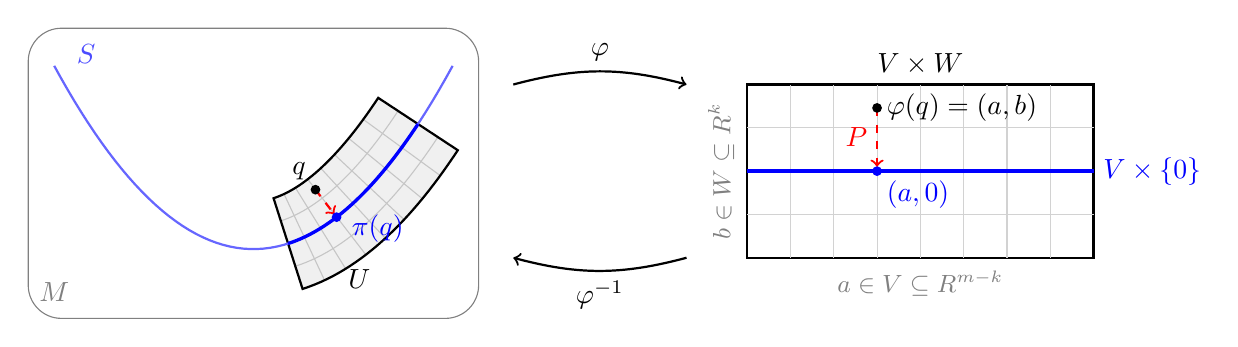
\begin{tikzpicture}[scale=1.1,
  declare function={nx(\u)=-0.8*\u/sqrt(1+0.64*\u*\u); ny(\u)=1/sqrt(1+0.64*\u*\u);
                    fx(\u,\v)=\u+\v*nx(\u); fy(\u,\v)=0.4*\u*\u+\v*ny(\u);}]
  \begin{scope}[yshift=-0.9cm]
    \draw[gray,rounded corners=12pt] (-2.6,-0.8) rectangle (2.6,2.55);
    \node[gray] at (-2.3,-0.5) {$M$};
    \fill[gray!12]
      plot[domain=0.4:1.9,samples=30,variable=\t] ({fx(\t,-0.55)},{fy(\t,-0.55)}) --
      plot[domain=-0.55:0.55,samples=10,variable=\t] ({fx(1.9,\t)},{fy(1.9,\t)}) --
      plot[domain=1.9:0.4,samples=30,variable=\t] ({fx(\t,0.55)},{fy(\t,0.55)}) --
      plot[domain=0.55:-0.55,samples=10,variable=\t] ({fx(0.4,\t)},{fy(0.4,\t)}) -- cycle;
    \foreach \c in {0.5875,0.775,0.9625,1.15,1.3375,1.525,1.7125}
      \draw[gray!45] plot[domain=-0.55:0.55,samples=10,variable=\t] ({fx(\c,\t)},{fy(\c,\t)});
    \foreach \c in {-0.275,0.275}
      \draw[gray!45] plot[domain=0.4:1.9,samples=30,variable=\t] ({fx(\t,\c)},{fy(\t,\c)});
    \draw[thick]
      plot[domain=0.4:1.9,samples=30,variable=\t] ({fx(\t,-0.55)},{fy(\t,-0.55)}) --
      plot[domain=-0.55:0.55,samples=10,variable=\t] ({fx(1.9,\t)},{fy(1.9,\t)}) --
      plot[domain=1.9:0.4,samples=30,variable=\t] ({fx(\t,0.55)},{fy(\t,0.55)}) --
      plot[domain=0.55:-0.55,samples=10,variable=\t] ({fx(0.4,\t)},{fy(0.4,\t)}) -- cycle;
    \node[below] at ({fx(0.9,-0.55)},{fy(0.9,-0.55)}) {$U$};
    \draw[thick,blue!60] plot[domain=-2.3:2.3,samples=60,variable=\t] ({\t},{0.4*\t*\t});
    \draw[very thick,blue] plot[domain=0.4:1.9,samples=30,variable=\t] ({\t},{0.4*\t*\t});
    \node[blue!70,right] at (-2.15,2.25) {$S$};
    \draw[red,thick,dashed,->] plot[domain=0.4:0.04,samples=10,variable=\t] ({fx(0.96,\t)},{fy(0.96,\t)});
    \fill ({fx(0.96,0.4)},{fy(0.96,0.4)}) circle (1.6pt) node[above left] {$q$};
    \fill[blue] (0.96,0.3686) circle (1.6pt) node[right,xshift=2pt,yshift=-4pt] {$\pi(q)$};
  \end{scope}
  \begin{scope}[xshift=7.7cm]
    \draw[thick] (-2,-1) rectangle (2,1);
    \foreach \c in {-1.5,-1,-0.5,0,0.5,1,1.5} \draw[gray!35] (\c,-1) -- (\c,1);
    \foreach \c in {-0.5,0.5} \draw[gray!35] (-2,\c) -- (2,\c);
    \draw[very thick,blue] (-2,0) -- (2,0);
    \node[blue,right] at (2,0) {$V \times \{0\}$};
    \draw[red,thick,dashed,->] (-0.5,0.73) -- (-0.5,0.05);
    \node[red,left] at (-0.5,0.39) {$P$};
    \fill (-0.5,0.73) circle (1.6pt) node[right] {$\varphi(q) = (a,b)$};
    \fill[blue] (-0.5,0) circle (1.6pt) node[below right] {$(a,0)$};
    \node[above] at (0,1) {$V \times W$};
    \node[gray] at (0,-1.3) {\small $a \in V \subseteq \mathbb{R}^{m-k}$};
    \node[gray,rotate=90] at (-2.3,0) {\small $b \in W \subseteq \mathbb{R}^{k}$};
  \end{scope}
  \draw[->,thick] (3.0,1.0) to[bend left=15] node[above] {$\varphi$} (5.0,1.0);
  \draw[->,thick] (5.0,-1.0) to[bend left=15] node[below] {$\varphi^{-1}$} (3.0,-1.0);
\end{tikzpicture}
